\documentclass[12pt,a4paper]{report}
\usepackage[brazil]{babel}
\usepackage[]{algorithm}
\usepackage[]{algorithmic}
\usepackage[style=numeric,backend=biber]{biblatex}
\usepackage[utf8]{inputenc}
\usepackage{kpfonts}
\usepackage[T1]{fontenc}
\usepackage{wrapfig}
\usepackage{graphicx}
\usepackage{enumerate}
\usepackage{subcaption}
\usepackage{float}
\usepackage{caption}
\usepackage{listings}
\usepackage{lipsum}
\usepackage{amsthm}
\usepackage{amssymb}
\usepackage{bm}
\usepackage{color}
\usepackage{afterpage}
\usepackage[inline]{enumitem}
\usepackage{pdflscape}
\usepackage{listingsutf8}
\usepackage{siunitx}
\usepackage{bashful}

\graphicspath{ {./images/} }

\lstset{frame=tb,
  aboveskip=2mm,
  belowskip=2mm,
  showstringspaces=false,
  columns=flexible,
  basicstyle=\footnotesize,,
  numbers=left,
  numbersep=5pt,
  stepnumber=1,
  breaklines=true,
  keepspaces=true,
  breakatwhitespace=true,
  showtabs=false,  
  tabsize=2
}

% Definindo estilo para os códigos
\definecolor{mGreen}{rgb}{0,0.6,0}
\definecolor{mGray}{rgb}{0.5,0.5,0.5}
\definecolor{mPurple}{rgb}{0.58,0,0.82}
\definecolor{dkgreen}{rgb}{0,0.6,0}
\definecolor{backgroundColour}{rgb}{0.97,0.97,0.97}

\lstset{basicstyle=\ttfamily,
    backgroundcolor=\color{backgroundColour},   
    commentstyle=\color{mGreen},
    keywordstyle=\color{magenta},
    numberstyle=\tiny\color{mGray},
    commentstyle=\color{dkgreen},
    stringstyle=\color{mPurple},
    basicstyle=\footnotesize,
    breakatwhitespace=false\textbf{,}         
    breaklines=true,                 
    captionpos=b,                    
    keepspaces=true,                 
    numbers=left,                    
    numbersep=5pt,                  
    showspaces=false,                
    showstringspaces=false,
    showtabs=false,                  
    tabsize=2,
    language=bash
}

\lstdefinestyle{BStyle}{
    backgroundcolor=\color{backgroundColour},  
    showstringspaces=false,
    numbers=none,
    language=bash
}

\pagenumbering{arabic}
\renewcommand{\thesection}{\arabic{section}}

\bibliography{ref}
\renewcommand{\contentsname}{Sumário}{\thispagestyle{empty}}
\renewcommand{\baselinestretch}{1.5} 

\begin{document}

\begin{titlepage}
    \begin{center}
        \vspace*{1cm}
        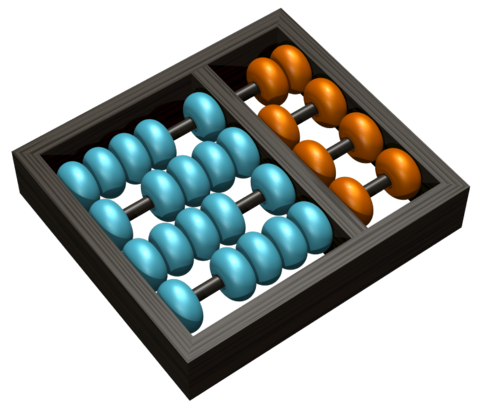
\includegraphics[width=0.25\textwidth]{Logo}\\
        \vspace{1.5cm}
        \Huge
    	\textbf{MC833 Relatório 5 \\
        Backlog e Processos Zumbis} \\
        \vspace{1.5cm}
        \Large
        \textbf{Aluno}: Fábio Camargo Ricci\\
        \textbf{RA}: 170781\\
        \vspace{1.2cm}
    	\Large 
    	Instituto de Computação\\
    	Universidade Estadual de Campinas\\
    	\vspace{1.5cm}
        Campinas, 09 de Novembro de 2021.
    \end{center}
\end{titlepage}
\tableofcontents
\clearpage

\newcommand{\shellcmd}[1]{\texttt{\footnotesize\# #1}}%estilizando citação de comandos do shell

\section{Questões}

\begin{enumerate}
    \item Explique o qué é multiplexação de E/S e faça um resumo das diferenças entre os 5 tipos de E/S.

    \item Modifique o programa cliente da atividade 3.2 para que este receba como entrada e envie ao servidor linhas de um arquivo texto qualquer. Explique no relatório as mudanças que considera mais importantes para sua solução.
    \begin{enumerate}
        \item O arquivo de texto de entrada será passado utilizando o caracter de
        redirecionamento '<'
        \item O cliente continuará recebendo o eco enviado pelo servidor, que deverá ser
        escrito em um arquivo. Esse arquivo será criado utilizando o caracter de
        redirecionamento '>'.
        \item Seu programa deverá necessariamente utilizar ou a função select ou a função
        poll.
        \item Cada linha deve ser enviada separadamente para o servidor. O servidor irá
        enviá-las de volta para o cliente, então cuidado com os ‘\textbackslash n’ e ‘\textbackslash t’.
        \item O cliente deve finalizar sua execução assim que tiver recebido todo o arquivo
        ecoado pelo servidor. Na saída padrão do servidor deve imprimir informações
        do cliente quando o cliente finalizar sua execução.
    \end{enumerate}
    
    \item Segundo o observado na solução do ponto 2, explique qual a limitação de usar a função close para fechar a conexão e qual a vantagem de usar a função shutdown no seu lugar.
\end{enumerate}

\section{Respostas}

\begin{enumerate}
    \item Se trata da capacidade de avisar o kernel que o processo deseja ser notificado quando condições de E/S (entrada e saída) estejam válidas (ex: dados para leitura estão disponíveis). Os 5 tipos de E/S são:
    \begin{enumerate}
        \item E/S bloqueante: Quando um processo faz a chamada de sistema, o mesmo é bloqueado e retorna a execução somente quando os recursos requisitados estiverem disponíveis.
        
        \item E/S não bloqueante: Quando um processo faz a chamada de sistema, o kernel retorna o erro EWOULDBLOCK caso os recursos não estejam disponíveis ou OK caso estejam.
        
        \item Multiplexação de E/S: Bloqueia o processo quando uma ou mais condições de E/S estão prontas para utilização, por ex: \\
        Primeiramente é chamado um \textbf{select()} que bloqueia o processo até os recursos estiverem disponíveis e retorna "readable". Após isso, o mesmo faz a chamada de sistema \textbf{recvfrom()} que o bloqueia novamente até a copia dos dados do kernel para o usuário ser finalizada.
        
        \item E/S orientada a sinal: O processo solicita ao kernel que notifique quando um evento ocorrer através do sinal \textbf{SIGIO}. Não é uma chamada bloqueante.
        
        \item E/S assíncrona: É uma chamada de sistema assíncrona não bloqueante, informando ao kernel que realize a operação e copie os dados do mesmo para o usuário. Notifica o processo quando toda a operação for finalizada.
    \end{enumerate}
    
    \item O cliente foi modificado para ler o input da entrada padrão, enviar os comandos para o servidor e imprimir os resultados na saída padrão. 
    \\
    Como o cliente trabalha com I/O na leitura do arquivo de entrada e na troca de mensagens com o servidor, utilizou-se a função \textbf{select()} para a multiplexação de I/O. Ao chamar a função \textbf{FD\_SET(fd)}, o processo indica ao kernel do SO que deseja ser notificado quando houver operações de I/O no file descriptor (fd) em questão. Dessa forma, sempre que houver uma operação de I/O basta utilizar a função \textbf{FD\_ISSET()} para verificar sobre qual file descriptor aquela operação se trata. 
    \\\\
    O código que trata essa lógica é o seguinte:
    \\
    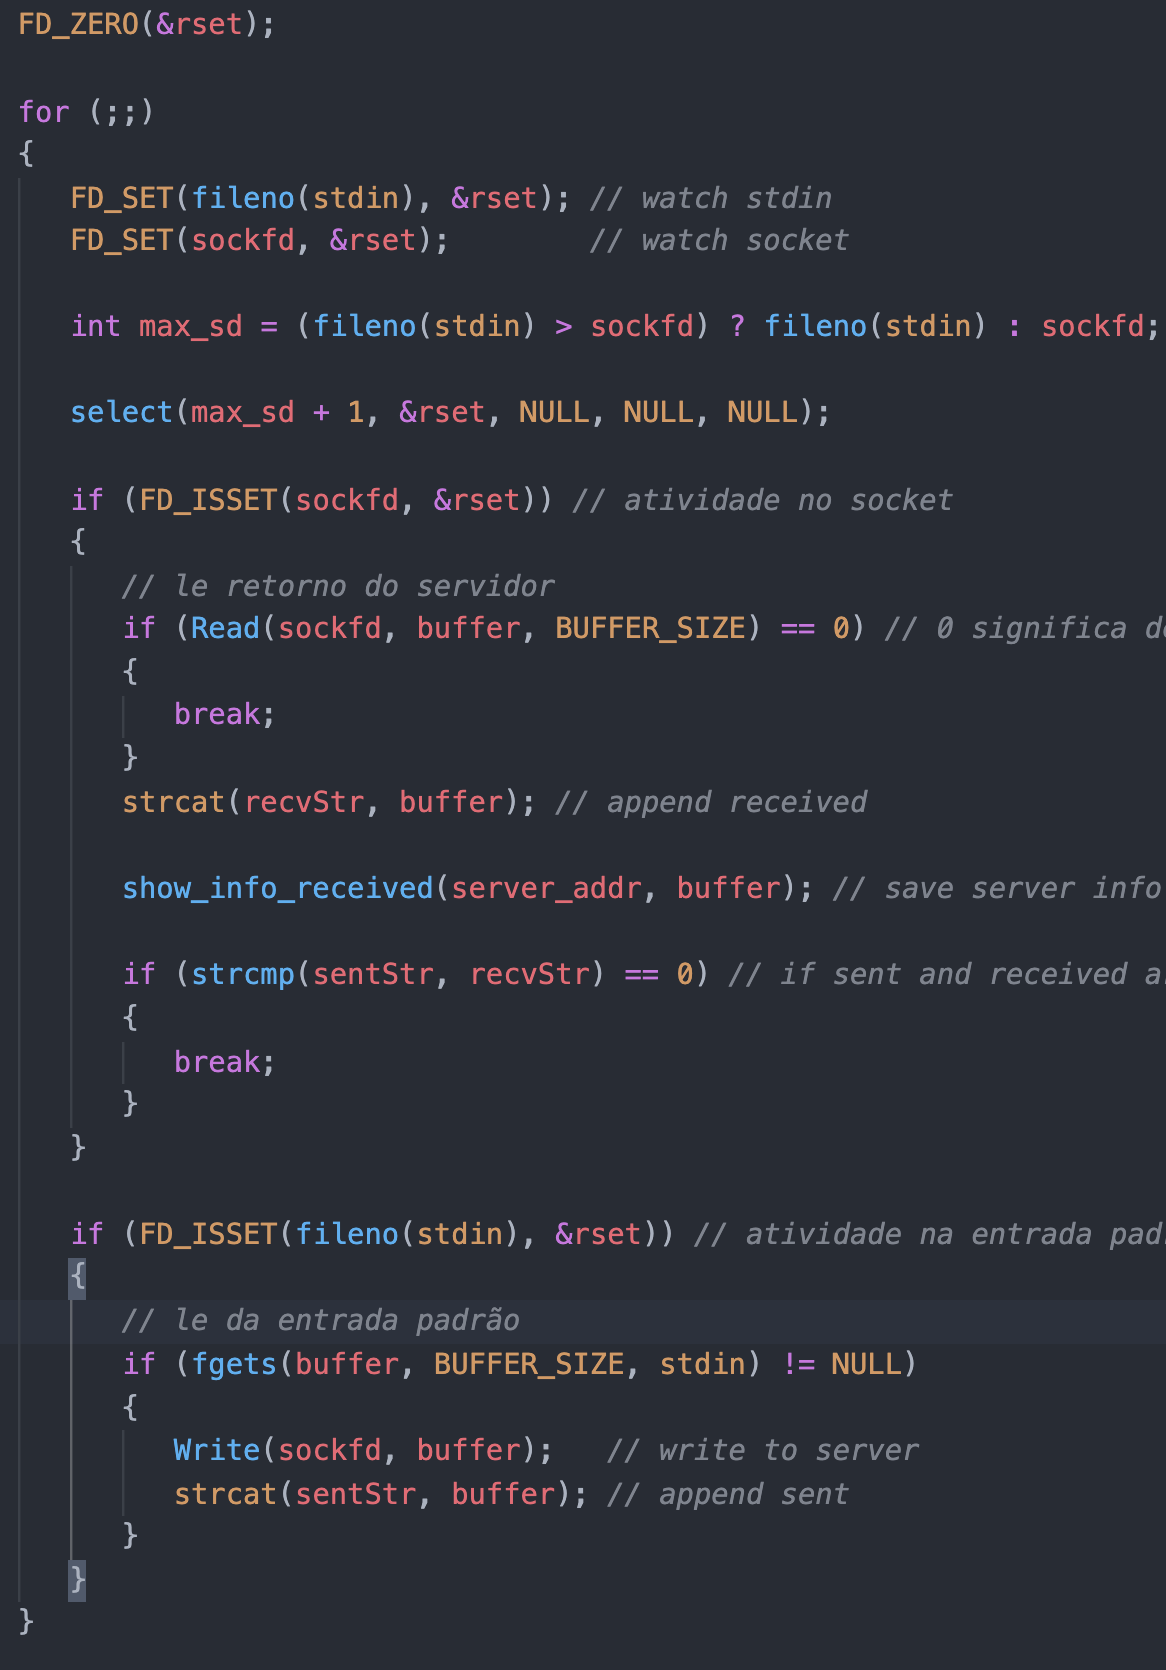
\includegraphics[width=\textwidth]{images/servidor-codigo.png}
    Com isso, redirecionando a entrada e saída padrão do cliente para os arquivos in.txt e out.txt respectivamente, compilou-se e executou-se o servidor e o cliente ():
    \\
    in.txt:\\\\
    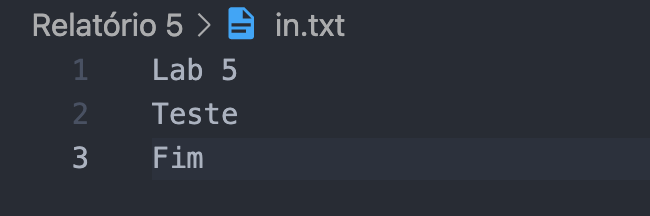
\includegraphics[width=\textwidth]{images/in.png}
    Servidor:\\\\
    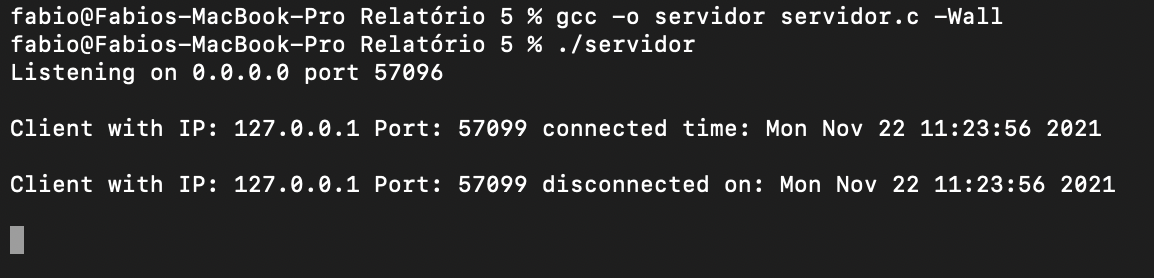
\includegraphics[width=\textwidth]{images/servidor.png}
    Cliente:\\\\
    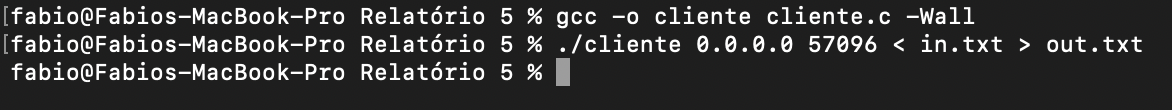
\includegraphics[width=\textwidth]{images/cliente.png}
    out.txt:\\\\
    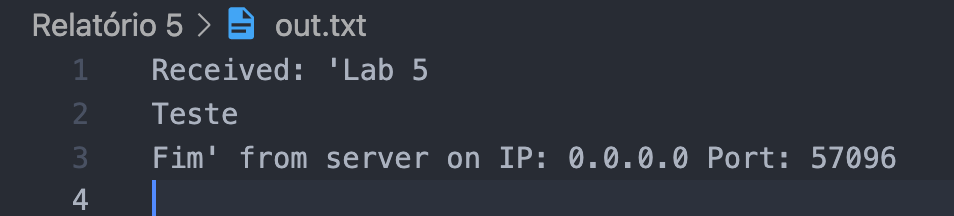
\includegraphics[width=\textwidth]{images/out.png}
    
    Para compilar os programas, utilizou-se os comandos:\\
    \textit{gcc -o servidor servidor.c -Wall}\\
    \textit{gcc -o cliente cliente.c -Wall}\\
    
    Para executar os programas, utilizou-se os comandos:\\
    \textit{./servidor}\\
    \textit{./cliente IP\_SERVIDOR PORTA\_SERVIDOR < in.txt > out.txt}\\
    
    Vale notar que colocou-se uma limitação do tamanho do arquivo de entrada de 40960 bytes (10 * BUFFER\_SIZE).
    
    \item As funções \textbf{close()} e \textbf{shutdown()} funcionam de maneiras diferentes:
    \begin{enumerate}
        \item close(): Bloqueia a comunicação com o socket o o destrói (termina suas conexões e destrói o file descriptor que habilita troca de mensagens). Toda mensagem trocada com esse socket após isso resultará em uma exceção ao processo.
        
        \item shutdown(): Bloqueia a comunicação com um socket sem que o mesmo seja destruído e recebe um parâmetro \textbf{how} que determina seu funcionamento:
        \begin{enumerate}
            \item \textbf{SHUT\_RD}: Bloqueia o socket de receber mensagens. Apesar disso, processos que leem do mesmo ainda podem ler dados no buffer (após isso, apenas reeberão mensagens vazias).
            
            \item \textbf{SHUT\_WR}: Bloqueia o socket de enviar mensagens. O mesmo também informa aos clientes conectados que o envio de mensagens está suspenso.
            
            \item \textbf{SHUT\_RDWR}: Bloqueia o socket de receber e enviar mensagens. Possui o mesmo funcionamento que chamar \textbf{shutdown(sockfd, SHUT\_RD)} e \textbf{shutdown(sockfd, SHUT\_WR)} em seguida
        \end{enumerate}
    \end{enumerate}
    
    Dessa forma, ao usar \textbf{shutdown}, o cliente e servidor podem indicar um ao outro que estão finalizando comunicações para que a contraparte possa tomar as ações apropriadas (vale notar que essa função não destrói o socket). A função \textbf{close} irá destruir o socket e finalizar a conexão no momento que é chamada, de modo que a contraparte irá receber um erro ao tentar se comunicar via o socket destruído novamente, não sendo possível, em alguns casos, fazer o encerramento armonioso da conexão entre as duas partes.
\end{enumerate}

\end{document}
